\chapter{Vectores}

\section{Sistemas de Coordenadas}
\subsection{Composición}

Un Sistema de Coordenadas se compone de:
\begin{itemize}
    \item Un origen
    \item Conjunto de ejes
    \item Instrucciones
\end{itemize}
\\
El primer uso de cualquier sistema de coordenadas es ubicar puntos en el espacio.

\newpage
\subsection{En el plano}
\textbf{Sistema de Coordenadas Rectangular}

\textbf{Ejemplo:} Ubicar los siguientes puntos en el S.C. rectangular:
\[
(x, y): A(5,4), \; B(4,5), \; C(-2,3), \; D(2,-3), \; E(-2,-3), \; F(4,-5)
\]

\subsection{Gráfico}

\begin{center}
\begin{tikzpicture}[scale=1]
    % Ejes
    \draw[->] (-4.5, 0) -- (5.5, 0) node[right] {$x$};
    \draw[->] (0, -5.5) -- (0, 5.5) node[above] {$y$};
    
    % Etiqueta del origen
    \node at (0.3, -0.3) {$O$};
    
    % Líneas de la cuadrícula
    \draw[dashed] (0, 4) -- (5, 4); % Línea horizontal A
    \draw[dashed] (5, 0) -- (5, 4); % Línea vertical A
    
    \draw[dashed] (0, 5) -- (4, 5); % Línea horizontal B
    \draw[dashed] (4, 0) -- (4, 5); % Línea vertical B
    
    \draw[dashed] (0, 3) -- (-2, 3); % Línea horizontal C
    \draw[dashed] (-2, 0) -- (-2, 3); % Línea vertical C
    
    \draw[dashed] (0, -3) -- (2, -3); % Línea horizontal D
    \draw[dashed] (2, 0) -- (2, -3); % Línea vertical D
    
    \draw[dashed] (0, -3) -- (-2, -3); % Línea horizontal E
    \draw[dashed] (-2, 0) -- (-2, -3); % Línea vertical E
    
    \draw[dashed] (0, -5) -- (4, -5); % Línea horizontal F
    \draw[dashed] (4, 0) -- (4, -5); % Línea vertical F
    
    % Puntos
    \filldraw (5,4) circle (2pt) node[above right] {$A$};
    \filldraw (4,5) circle (2pt) node[above right] {$B$};
    \filldraw (-2,3) circle (2pt) node[above left] {$C$};
    \filldraw (2,-3) circle (2pt) node[below right] {$D$};
    \filldraw (-2,-3) circle (2pt) node[below left] {$E$};
    \filldraw (4,-5) circle (2pt) node[below right] {$F$};
    
    % Numeración de los ejes
    \foreach \x in {-4, -3, -2, -1, 1, 2, 3, 4, 5}
        \draw (\x, -0.1) -- (\x, 0.1) node[below] {\x};
    \foreach \y in {-5, -4, -3, -2, -1, 1, 2, 3, 4, 5}
        \draw (-0.1, \y) -- (0.1, \y) node[left] {\y};
\end{tikzpicture}
\end{center}

\newpage
\section{Sistema de Coordenadas Polar}

Un sistema de coordenadas polares define un punto $P(r, \theta)$ mediante:
\begin{itemize}
    \item $r$: La distancia entre el punto $P$ y el origen $O$.
    \item $\theta$: El ángulo entre el eje polar (eje positivo $x$) y la línea que conecta $P$ con el origen, medido en sentido antihorario.
\end{itemize}

\begin{center}
\begin{tikzpicture}[scale=1.5]
    % Ejes
    \draw[->] (-1, 0) -- (3, 0) node[right] {$x$};
    \draw[->] (0, -1) -- (0, 3) node[above] {$y$};
    
    % Punto P
    \draw[dashed] (0, 0) -- (2, 1.5) node[midway, above] {$r$};
    \filldraw (2, 1.5) circle (1pt) node[right] {$P(r, \theta)$};
    
    % Ángulo theta
    \draw[->] (0.5, 0) arc (0:36.87:0.5);
    \node at (0.8, 0.2) {$\theta$};
\end{tikzpicture}
\end{center}

\newpage
\section{Coordenada Angular}

La coordenada angular $\theta$ puede expresarse en grados o en radianes. A continuación, se presentan ambos sistemas de referencia.

\subsection*{En Grados}
\begin{center}
\begin{tikzpicture}[scale=1.5]
    % Ejes
    \draw[->] (-2, 0) -- (2, 0) node[right] {$0^\circ$ o $360^\circ$};
    \draw[->] (0, -2) -- (0, 2) node[above] {$90^\circ$};
    \draw[->] (0, 0) -- (-2, 0) node[left] {$180^\circ$};
    \draw[->] (0, 0) -- (0, -2) node[below] {$270^\circ$};
\end{tikzpicture}
\end{center}

\subsection*{En Radianes}
\begin{center}
\begin{tikzpicture}[scale=1.5]
    % Ejes
    \draw[->] (-2, 0) -- (2, 0) node[right] {$0$ o $2\pi$};
    \draw[->] (0, -2) -- (0, 2) node[above] {$\frac{\pi}{2}$};
    \draw[->] (0, 0) -- (-2, 0) node[left] {$\pi$};
    \draw[->] (0, 0) -- (0, -2) node[below] {$\frac{3\pi}{2}$};
\end{tikzpicture}
\end{center}

\newpage
\section{Equivalencia}

\subsection{Equivalencia entre las unidades}
Se tiene la siguiente equivalencia fundamental:
\[
    180^{\circ} = \pi \text{ rad}
\]
Para convertir de grados a radianes, se usa la relación:
\[
x^{\circ} = x \left( \frac{\pi \text{ rad}}{180^{\circ}} \right)
\]
Por ejemplo, si se desea convertir $60^{\circ}$ a radianes:
\[
60^{\circ} = 60 \left( \frac{\pi}{180} \right) = \frac{\pi}{3} \text{ rad}\]

\newpage
\section{Cantidades Escalares \& Vectoriales}

\subsection{Cantidad Escalar}
Se especifica por un valor numérico y una unidad.

\subsection{Cantidad Vectorial}
Se especifica por un valor numérico, una unidad y una dirección.

\section{Propiedades}

\subsection{Igualdad de Vectores}
Dos vectores $\vec{A}$ y $\vec{B}$ son iguales si:
\[
    \vec{A} = \vec{B} \quad \text{y} \quad |\vec{A}| = |\vec{B}| \quad \text{con igualdad de dirección.}
\]

\subsection{Representación Gráfica de la Igualdad}
\begin{center}
    \begin{tikzpicture}[scale=1]
        % Vector A
        \draw[->] (0,0) -- (2,1) node[midway, above] {$\vec{A}$};
        
        % Vector B
        \draw[->] (4,0) -- (6,1) node[midway, above] {$\vec{B}$};
    \end{tikzpicture}
\end{center}

\subsection{Suma de Vectores}
\begin{center}
    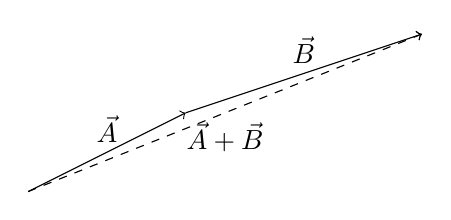
\begin{tikzpicture}[scale=1]
        % Vector A
        \draw[->] (0,0) -- (2,1) node[midway, above] {$\vec{A}$};
        
        % Vector B desde el extremo de A
        \draw[->] (2,1) -- (5,2) node[midway, above] {$\vec{B}$};
        
        % Vector A + B
        \draw[->, dashed] (0,0) -- (5,2) node[midway, below] {$\vec{A} + \vec{B}$};
    \end{tikzpicture}
\end{center}

\newpage
\section{Propiedades de la Suma}
\begin{itemize}
    \item \textbf{Conmutativa:}
    \[
    \vec{A} + \vec{B} = \vec{B} + \vec{A}
    \]

    \item \textbf{Elemento Neutro:}
    \[
    \vec{A} + \vec{0} = \vec{A}
    \]

    \item \textbf{Negatividad:}
    \[
    \vec{A} + (-\vec{A}) = \vec{0}
    \]

    \item \textbf{Asociatividad:}
    \[
    (\vec{A} + \vec{B}) + \vec{C} = \vec{A} + (\vec{B} + \vec{C})
    \]

    \item \textbf{Multiplicación por un escalar:}
    \[
    c \vec{A}
    \]
\end{itemize}

\newpage
\section{Vectores Unitarios}

\subsection{Definición}

Los \textbf{vectores unitarios} son vectores adimensionales, de módulo (o magnitud) y solo indican una dirección.
\\[0.5cm]
Se puede construir vectores unitarios a partir de cualquier vector $\vec{a}$:
\[
\hat{a} = \frac{\vec{a}}{|\vec{a}|},
\]
\\
donde $\hat{a}$ es el vector unitario en la dirección de $\vec{a}$.

\subsection{Uso de vectores unitarios}

A menudo se utilizan vectores unitarios en la dirección de los ejes del sistema de coordenadas :
\begin{itemize}
    \item $\hat{i}$ (Eje $x$),
    \item $\hat{j}$ (Eje $y$),
    \item $\hat{k}$ (Eje $z$).
\end{itemize}
\\
Cualquier vector $\vec{A}$ se puede expresar como:
\[
\vec{A} = A_x \hat{i} + A_y \hat{j},
\]
\\
donde $A_x$ y $A_y$ son las componentes del vector en las direcciones $x$ e $y$, respectivamente.

\subsection{Suma de vectores}

Dados dos vectores:
\begin{align*}
\vec{A} &= A_x \hat{i} + A_y \hat{j}, \\
\vec{B} &= B_x \hat{i} + B_y \hat{j},
\end{align*}
\\
su suma es:
\[
\vec{A} + \vec{B} = (A_x + B_x)\hat{i} + (A_y + B_y)\hat{j}.
\]

\newpage
\subsection{Gráfico}
El siguiente gráfico representa un vector $\vec{A}$ en el plano:

\begin{center}
\begin{tikzpicture}[scale=1]
    % Ejes coordenados
    \draw[->] (-0.5,0) -- (4,0) node[right] {$x$};
    \draw[->] (0,-0.5) -- (0,4) node[above] {$y$};

    % Vector A
    \draw[->, thick] (0,0) -- (3,2) node[midway, above] {$\vec{A}$};

    % Etiquetas
    \node at (3.2,0) [below] {$A_x$};
    \node at (0,2.2) [left] {$A_y$};

    % Proyecciones
    \draw[dashed] (3,2) -- (3,0);
    \draw[dashed] (3,2) -- (0,2);
\end{tikzpicture}
\end{center}

\subsection{Producto escalar}

El producto escalar de dos vectores $\vec{A}$ y $\vec{B}$ se define como:
\[
\vec{A} \cdot \vec{B} = |\vec{A}| |\vec{B}| \cos\varphi,
\]
\\
donde $\varphi$ es el ángulo entre $\vec{A}$ y $\vec{B}$.

\begin{itemize}
    \item Si $\vec{A} \cdot \vec{B} > 0$, entonces $0 \leq \varphi < 90^\circ$:
    \begin{center}
    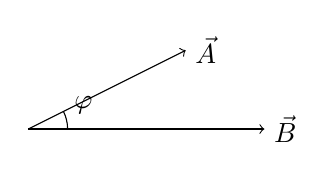
\begin{tikzpicture}[scale=1]
        \draw[->] (0,0) -- (3,0) node[right] {$\vec{B}$};
        \draw[->] (0,0) -- (2,1) node[right] {$\vec{A}$};
        \draw (0.5,0) arc[start angle=0, end angle=26.57, radius=0.5];
        \node at (0.7,0.3) {$\varphi$};
    \end{tikzpicture}
    \end{center}

    \item Si $\vec{A} \cdot \vec{B} = 0$, entonces $\varphi = 90^\circ$:
    \begin{center}
    \begin{tikzpicture}[scale=1]
        \draw[->] (0,0) -- (3,0) node[right] {$\vec{B}$};
        \draw[->] (0,0) -- (0,2) node[above] {$\vec{A}$};
        \draw (0.5,0) arc[start angle=0, end angle=90, radius=0.5];
        \node at (0.3,0.3) {$90^\circ$};
    \end{tikzpicture}
    \end{center}

    \item Si $\vec{A} \cdot \vec{B} < 0$, entonces $90^\circ < \varphi \leq 180^\circ$:
    \begin{center}
    \begin{tikzpicture}[scale=1]
        \draw[->] (0,0) -- (3,0) node[right] {$\vec{B}$};
        \draw[->] (0,0) -- (-2,1) node[left] {$\vec{A}$};
        \draw (0.5,0) arc[start angle=0, end angle=153.43, radius=0.5];
        \node at (-0.5,0.5) {$\varphi$};
    \end{tikzpicture}
    \end{center}
\end{itemize}

\section{Producto Escalar Usando Componentes}
El producto escalar entre dos vectores se define como:
\[
\vec{A} \cdot \vec{B} = A_x B_x + A_y B_y + A_z B_z.
\]

\subsection{Ejemplo}
Efectuar el producto escalar entre los vectores:
\begin{align*}
\vec{A} &= 4\hat{i} + 5\hat{j} - 3\hat{k}, \\
\vec{B} &= -2\hat{i} + 4\hat{j} + 7\hat{k}.
\end{align*}

\subsubsection{Solución}
\begin{align*}
\vec{A} \cdot \vec{B} &= (4)(-2) + (5)(4) + (-3)(7) \\
&= -8 + 20 - 21 \\
&= -9 \quad \text{u.a.}
\end{align*}

\newpage
\section{Aplicacion de los productos vectoriales}

\subsection{Definición del Producto Vectorial}
El producto vectorial entre dos vectores $\vec{A}$ y $\vec{B}$ está definido como:
\begin{equation}
    |\vec{A} \times \vec{B}| = |\vec{A}| |\vec{B}| \sin \phi,
\end{equation}
donde $\phi$ es el ángulo entre los vectores $\vec{A}$ y $\vec{B}$. Su dirección es perpendicular al plano formado por $\vec{A}$ y $\vec{B}$.

\begin{center}
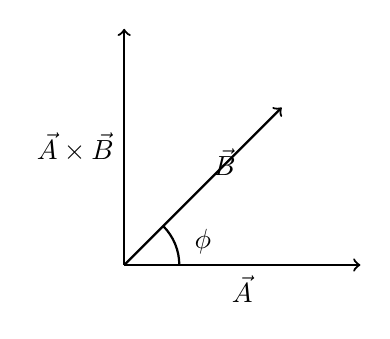
\begin{tikzpicture}
    % Vector A
    \draw[->, thick] (0,0) -- (3,0) node[midway, below] {$\vec{A}$};
    % Vector B
    \draw[->, thick] (0,0) -- (2,2) node[midway, above right] {$\vec{B}$};
    % Perpendicular vector (A x B)
    \draw[->, thick] (0,0) -- (0,3) node[midway, left] {$\vec{A} \times \vec{B}$};
    % Angle arc
    \draw[thick] (0.7,0) arc[start angle=0, end angle=45, radius=0.7cm];
    \node at (1, 0.3) {$\phi$};
\end{tikzpicture}
\end{center}

\subsection{Regla de la Mano Derecha}
La dirección del producto vectorial $\vec{A} \times \vec{B}$ se determina usando la regla de la mano derecha. Si:
\begin{itemize}
    \item Los dedos de la mano derecha apuntan en la dirección de $\vec{A}$,
    \item Y se curvan hacia $\vec{B}$,
    \item Entonces el pulgar señala la dirección de $\vec{A} \times \vec{B}$ (saliente del plano).
\end{itemize}

Si se invierte el orden de los vectores ($\vec{B} \times \vec{A}$), el producto vectorial apunta hacia dentro del plano.

\begin{center}
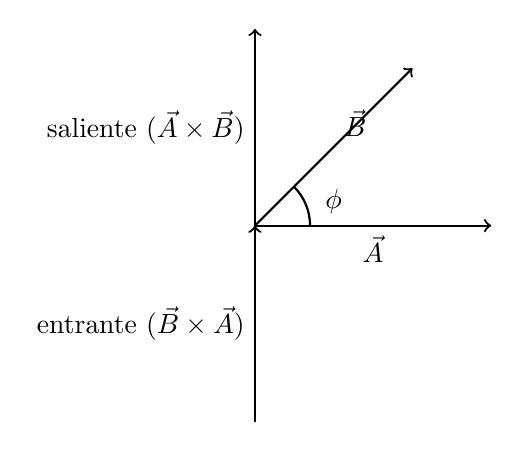
\begin{tikzpicture}
    % Vector A
    \draw[->, thick] (0,0) -- (3,0) node[midway, below] {$\vec{A}$};
    % Vector B
    \draw[->, thick] (0,0) -- (2,2) node[midway, above right] {$\vec{B}$};
    % Perpendicular vectors
    \draw[->, thick] (0,0) -- (0,2.5) node[midway, left] {saliente ($\vec{A} \times \vec{B}$)};
    \draw[<-, thick] (0,0) -- (0,-2.5) node[midway, left] {entrante ($\vec{B} \times \vec{A}$)};
    % Angle arc
    \draw[thick] (0.7,0) arc[start angle=0, end angle=45, radius=0.7cm];
    \node at (1, 0.3) {$\phi$};
\end{tikzpicture}
\end{center}

\section{Producto Vectorial Usando Componentes}
Si $\vec{A} = A_x \hat{i} + A_y \hat{j} + A_z \hat{k}$ y $\vec{B} = B_x \hat{i} + B_y \hat{j} + B_z \hat{k}$, entonces el producto vectorial se calcula como:
\begin{equation}
    \vec{A} \times \vec{B} = \begin{vmatrix}
        \hat{i} & \hat{j} & \hat{k} \\
        A_x & A_y & A_z \\
        B_x & B_y & B_z \\
    \end{vmatrix}.
\end{equation}

Esto se desarrolla como:
\begin{align}
    \vec{A} \times \vec{B} = &\, (A_y B_z - A_z B_y) \hat{i} + (A_z B_x - A_x B_z) \hat{j} + (A_x B_y - A_y B_x) \hat{k}.
\end{align}

\subsection{Producto por un Escalar}
\begin{align*}
    c\vec{A} &= c\big(A_x\hat{i} + A_y\hat{j} + A_z\hat{k}\big) \\
             &= cA_x\hat{i} + cA_y\hat{j} + cA_z\hat{k}
\end{align*}